\setcounter{page}{1} % Iniciar la numeración de las páginas en este punto

\section{Introducción}


\section{Antecedentes}

    \subsubsection*{A chest-based continuous cuffless blood pressure method: Estimation and evaluation using multiple body sensors \cite{bodySensor}.}

    El artículo analiza el desarrollo de un dispositivo no invasivo para la estimación de la presión arterial (PA) utilizando sensores colocados en el pecho utilizando la bioimpedancia (BImp) como alternativa a la fotopletismografía (PPG) para la extracción del tiempo de llegada del pulso (PAT), se tomaron cinco lecturas de tiempo de pulso diferentes y se pudo estimar la PA sistólica y diastólica. 
    
    Se analizaron los datos de 41 participantes en diversas condiciones fisiológicas, incluidos los cambios de postura y los resultados mostraron que la combinación de PAT con la frecuencia cardíaca 
    mejoró la precisión del cálculo de la PA, y las lecturas de PAT basadas en BImp fueron un 3\% más precisas que las basadas en PPG, lo que destaca el potencial de BImp para un control más eficaz de la PA.

    \subsubsection*{An Arterial Compliance Sensor for Cuffless Blood Pressure Estimation Based on Piezoelectric and Optical Signals \cite{piezoelectric}.}

    Este artículo propone el desarrollo de un pequeño sistema de monitoreo que integra una matriz de sensosres piezoeléctricos y un sensor óptico que monitorea las señales fisiológicas de la arteria radial. El sistema hace el cálculo del tiempo de tránsito del pulso (PTT) y correlaciona la ecuación de Moens-Korteweg con la velocidad de onda de pulso (PWV) para estimar la presión arterial sistólica (PAS) y diastólica (PAD).

    En un experimento con 20 participantes se compararon dos métodos de estimación de la presión arterial, el primero utilizando el modelo de regresión y el segundo modelo $P-\beta$ basado en la ecuación de Moens-Korteweg.

    \subsubsection*{Development of IoT Based Cuffless Blood Pressure Measurement System \cite{Norsuriati_2021}.}

    El artículo presenta el desarrollo de un sistema IoT de medición de presión arterial sin uso de un baumanómetro, se propone un método basado en el tiempo de tránsito del pulso (PTT). Este método correlaciona el tiempo de retraso entre las señales fotopletismografía (PPG) registrada en la punta del dedo y el lóbulo de la oreja.

    Los datos son recolectados mediante un microcontrolador Arduino Uno y procesados con el software MATLAB para eliminar el ruido y obtener los picos de la señal PPG para calcular el PTT.
    
    Los resultados son mostrados en la aplicación ThinkSpeak y ThingView debido a que tiene la capacidad de almacenar y visualizar los datos en tiempo real. El error medio y la deviación estándar para la presión arterial sistólica (PAS) estimada es de $22,5 \pm 20,6$ mmHg y para la presión arterial diastólica (PAD) es de $1,6 \pm 1,2$ mmHg.

    \subsubsection*{Diseño de un sistema internet de las cosas (IoT) para el monitoreo de la presión arterial \cite{Estrada_2021}. }

    En este artículo se presenta los procesos de diseño y construcción de un prototipo biomédico IoT para el monitoreo de la presión arterial de pacientes en su lugar de residencia. El sistema consta en colocar un brazalete al paciente a la altura del corazón, el cual se le conecta una bomba de aire el cual infla el brazalete y un sensor de presión diferencial MPX5050DP, se realiza una conversión análoga-digital con ayuda de un microcontrolador y se envía los datos meidante una API REST al servidor web IoT ThinkSpeak donde se almacenan y se pueden visualizar en tiempo real.

    \subsubsection*{Development of Real-Time Cuffless Blood Pressure Measurement Systems with ECG Electrodes and a Microphone Using Pulse Transit Time (PTT) \cite{Electrodes_Microphone}.}

    El estudio habla sobre el desarrollo de un sistema de medición de la presión arterial en tiempo real sin uso de un baumanómetro, utilizando electrodos de ECG y un micrófono en lugar de un sensor de fotopletismografía (PPG). El sistema mide la onda de pulso sanguíneo en la arteria radial de la muñeca, calculando la presión arterial sistólica (SBP) y diastólica (DBP) mediante el tiempo de tránsito del pulso (PTT) entre el pico R del ECG y puntos característicos de la onda de pulso.
    
    Las estimaciones de SBP y DBP fueron comparables a las de un monitor de presión arterial comercial, con un error absoluto medio (MAE) de $2.72 \pm 3.42$ mmHg para SBP y $2.29 \pm 3.53$ mmHg para DBP.


\newpage
\section{Justificación}

En México, las enfermedades cardiovasculares representan la primera causa de muerte, siendo responsable de más de 220 mil fallecimientos en 2021 \cite{SSFallecimientos}. Entre los factores de riesgo más importantes para estas patologías se encuentra la hipertensión arterial, conocida también como el ``asesino silencioso", ya que no presenta síntomas y puede pasar desapercibida durante años, hasta que desarrollan complicaciones graves como infartos o accidentes cerebrovasculares. Según la Encuesta Nacional de Salud y Nutrición (ENSANUT), cerca del 30\% de la población adulta en México padece hipertensión arterial \cite{ENSANUT}, pero una gran proporción de ellos no recibe un tratamiento adecuado o no se diagnostica a tiempo debido a la falta de acceso a un monitoreo continuo y preciso.

Los métodos para la medición de la presión arterial, como el baumanómetro, son invasivos y requieren de personal capacitado, lo que limita su uso en el monitoreo continuo de la presión arterial. Esta limitación es crítica en un país como México, donde el sistema de salud puede ser limitado, especialmente en zonas rurales y marginadas. Por lo tanto, es necesario desarrollar dispositivos no invasivos y de bajo coste que permitan a las personas el monitorear su presión arterial de forma continua y precisa, para detectar y tratar a tiempo la hipertensión arterial y de esta forma prevenir complicaciones graves.

Este proyecto tiene como objetivo desarrollar un sistema basado en sensores para la estimación de la presión arterial de forma no invasiva, que permita a las personas monitorear su presión arterial de forma continua y precisa, y enviar los datos a un dispositivo móvil para la visualización y el almacenamiento de los registros para llevar un control de su salud cardiovascular. Facilitando así la detección temprana de la hipertensión arterial y la prevención de complicaciones graves asociadas a esta enfermedad.

El desarrollo de un sistema de monitoreo no invasivo de la presión arterial permitirá a las personas tener un mayor control de su salud cardiovascular, detectar a tiempo la hipertensión arterial y prevenir complicaciones graves asociadas a esta enfermedad, mejorando así su calidad de vida y reduciendo la carga de enfermedades cardiovasculares en México.


\newpage
\section{Objetivos}
    \subsection{Objetivo General}
    Desarrollar un dispositivo para estimar la presión arterial de forma no invasiva utilizando sensores.
    \subsection{Objetivos Específicos}
    \begin{itemize}
        \item Diseñar un dispositivo utilizando sensores para la obtención de datos fisiológicos.
        \item Enviar los datos mediante Bluetooth a un dispositivo móvil.
        \item Implementar un algoritmo de procesamiento de señales para la estimación de la presión arterial.
        \item Visualizar los datos obtenidos en una aplicación android.
    \end{itemize}

\newpage
\section{Marco Teórico}

    \subsection{El sistema de conducción del corazón}

    El corazón es un músculo que late y bombea continuamente sangre al resto del cuerpo. Lo que comúnmente llamamos latido cardíaco es en realidad la contracción rítmica de las cuatro cavidades del corazón. Cada latido cardíaco es estimulado por señales eléctricas que viajan a través de una vía específica del corazón. Estas señales se pueden registrar mediante un electrocardiograma (ECG).

     Este proceso comienza en el nódulo senoauricular (nódulo SA), situado en la aurícula derecha. La señal eléctrica se propaga a las aurículas, provocando su contracción y el empuje de sangre hacia los ventrículos. Luego, la señal llega al nódulo auriculoventricular (nódulo AV) y se desplaza a través del haz de His, que se divide en ramas izquierda y derecha dentro de los ventrículos. Finalmente, la señal viaja por las fibras de Purkinje, que son fibras musculares especializadas que se encuentran en las paredes de los ventrículos, el cual provoca la contracción de los ventrículos, bombeando sangre a los pulmones y al resto del cuerpo. Este sistema actúa como el marcapasos natural del cuerpo, manteniendo un ritmo cardíaco normal de 60 a 100 latidos por minuto. Alteraciones en este sistema pueden resultar en ritmos cardíacos anormales y afectar el flujo sanguíneo del cerebro y otras partes del cuerpo \cite{SistemaConduccionMSD}.

    \begin{figure}[H]
        \centering
        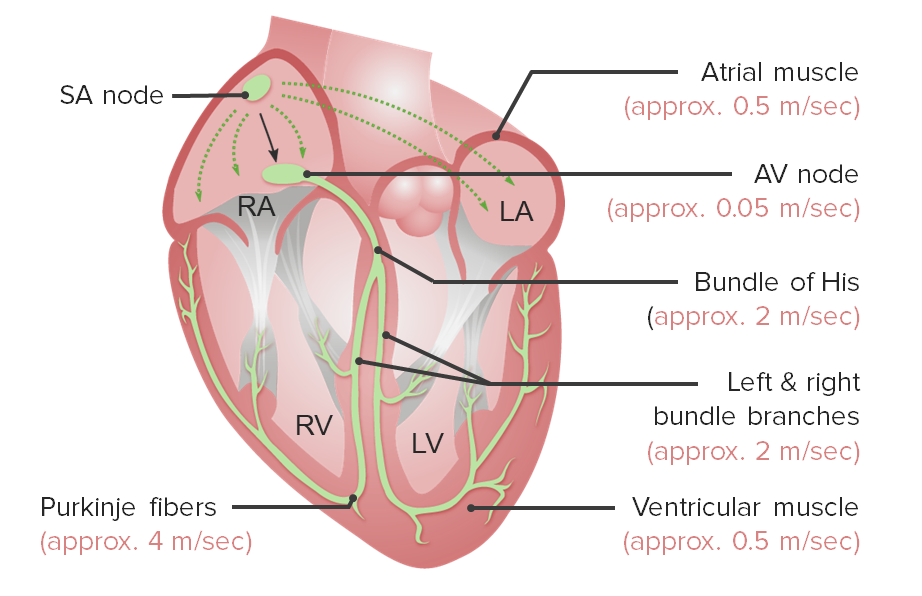
\includegraphics[width=0.8\textwidth]{img/sistemaConduccion.png}
        \caption[Sistema de conducción cardíaca y tiempos de conducción de los respectivos segmentos]{Sistema de conducción cardíaca y tiempos de conducción de los respectivos segmentos\footnotemark}
        \label{fig:sistemaConduccion}
    \end{figure}
    \footnotetext{Localización de las células marcapasos dentro del sistema de conducción del corazón. Imagen tomada de lecturio.com. Fuente: \url{https://goo.su/MSZMxUj}}

    \subsection{Electrocardiograma (ECG)}
    Un electrocardiograma (ECG) es un estudio que registra el voltaje generado por los vectores de despolarización y repolarización de las células cardiacas en relación con el tiempo, es una herramienta útil para evaluar la función cardíaca y detectar problemas cardíacos. \cite{ECG_Definicion}

    Es una prueba no invasiva e indolora, que se realiza para detectar problemas cardíacos o controlar el estado del corazon. El ECG generalmente utiliza sensores (electrodos), colocados sobre la piel del pecho, pueden detectar señales eléctricas del corazón. Las señales de estos sensores se conectan a circuitos electrónicos simples con amplificadores, filtros y convertidores analógico-digitales, que registran la señal eléctrica y la muestran en un monitor o la imprimen para su posterior análisis.

    Las ondas del ECG son las siguientes:

    \begin{itemize}
        \item \textbf{Onda P}: Representa la despolarización auricular, es la suma de los vectores de despolarización de ambas aurículas.
        \item \textbf{Intervalo PR}: Representa el tiempo transcurrido desde la despolarización auricular, hasta la despolarización ventricular. Incluye la onda P y el segmento PR. Éste último elemento es una línea isoeléctrica, establecida gracias al retardo fisiológico que sufre la conducción eléctrica en el nodo aurículoventricular. Sin este retraso mencionado, las aurículas y los ventrículos se despolarizarían casi al mismo tiempo, siendo imposible el funcionamiento correcto del corazón para que la sangre pase por sus diferentes cavidades ordenadamente.
        \item \textbf{Onda Q}: Indica el inicio de la despolarización ventricular, específicamente el vector de despolarización septal.
        \item \textbf{Onda R}: Representa el segundo vector de despolarización, correspondiente a la pared libre del ventrículo izquierdo. Es normalmente la onda con mayor voltaje, debido a que el ventrículo izquierdo es el que mayor cantidad de células posee, por ende, la actividad eléctrica es mayor y el vector es más grande.
        \item \textbf{Onda S}: Corresponde al último vector de despolarización ventricular, originado en las bases de los ventrículos.
        \item \textbf{Complejo QRS}: Es la suma de los tres vectores de despolarización anteriores, y juntos representan a la despolarización ventricular.
        \item \textbf{Segmento ST}: Es un periodo de inactividad que separa la despolarización ventricular de la repolarización ventricular, va desde el final del complejo QRS hasta el comienzo de la onda T. 
        \item \textbf{Intervalo QT}: Se extiende desde el comienzo del complejo QRS hasta el final de la onda T y representa la sístole eléctrica ventricular, o lo que es lo mismo, el conjunto de la despolarización y repolarización ventricular. La medida de este intervalo depende de la frecuencia cardiaca, de forma que el intervalo QT se acorta cuando la frecuencia cardiaca es alta, y se alarga cuando la frecuencia cardiaca es baja. Por lo anterior, cuando se mide, es necesario corregirlo de acuerdo con la frecuencia cardíaca utilizando la fórmula de Bazett
        \item \textbf{Onda T}: Es la onda que representa la repolarización ventricular.
        \item \textbf{Onda U}: Es una onda de escaso voltaje que puede o no estar presente en el trazado del electrocardiograma. Se debe a la repolarización de los músculos papilares
        \item \textbf{Intervalo RR}: Es el intervalo que abarca desde una onda R, hasta la onda R de la siguiente despolarización, es decir dos ondas R sucesivas. En un paciente sano, debe permanecer a un ritmo constante. La medida de este intervalo dependerá de la frecuencia cardiaca.
    \end{itemize}

    \begin{figure}[H]
        \centering
        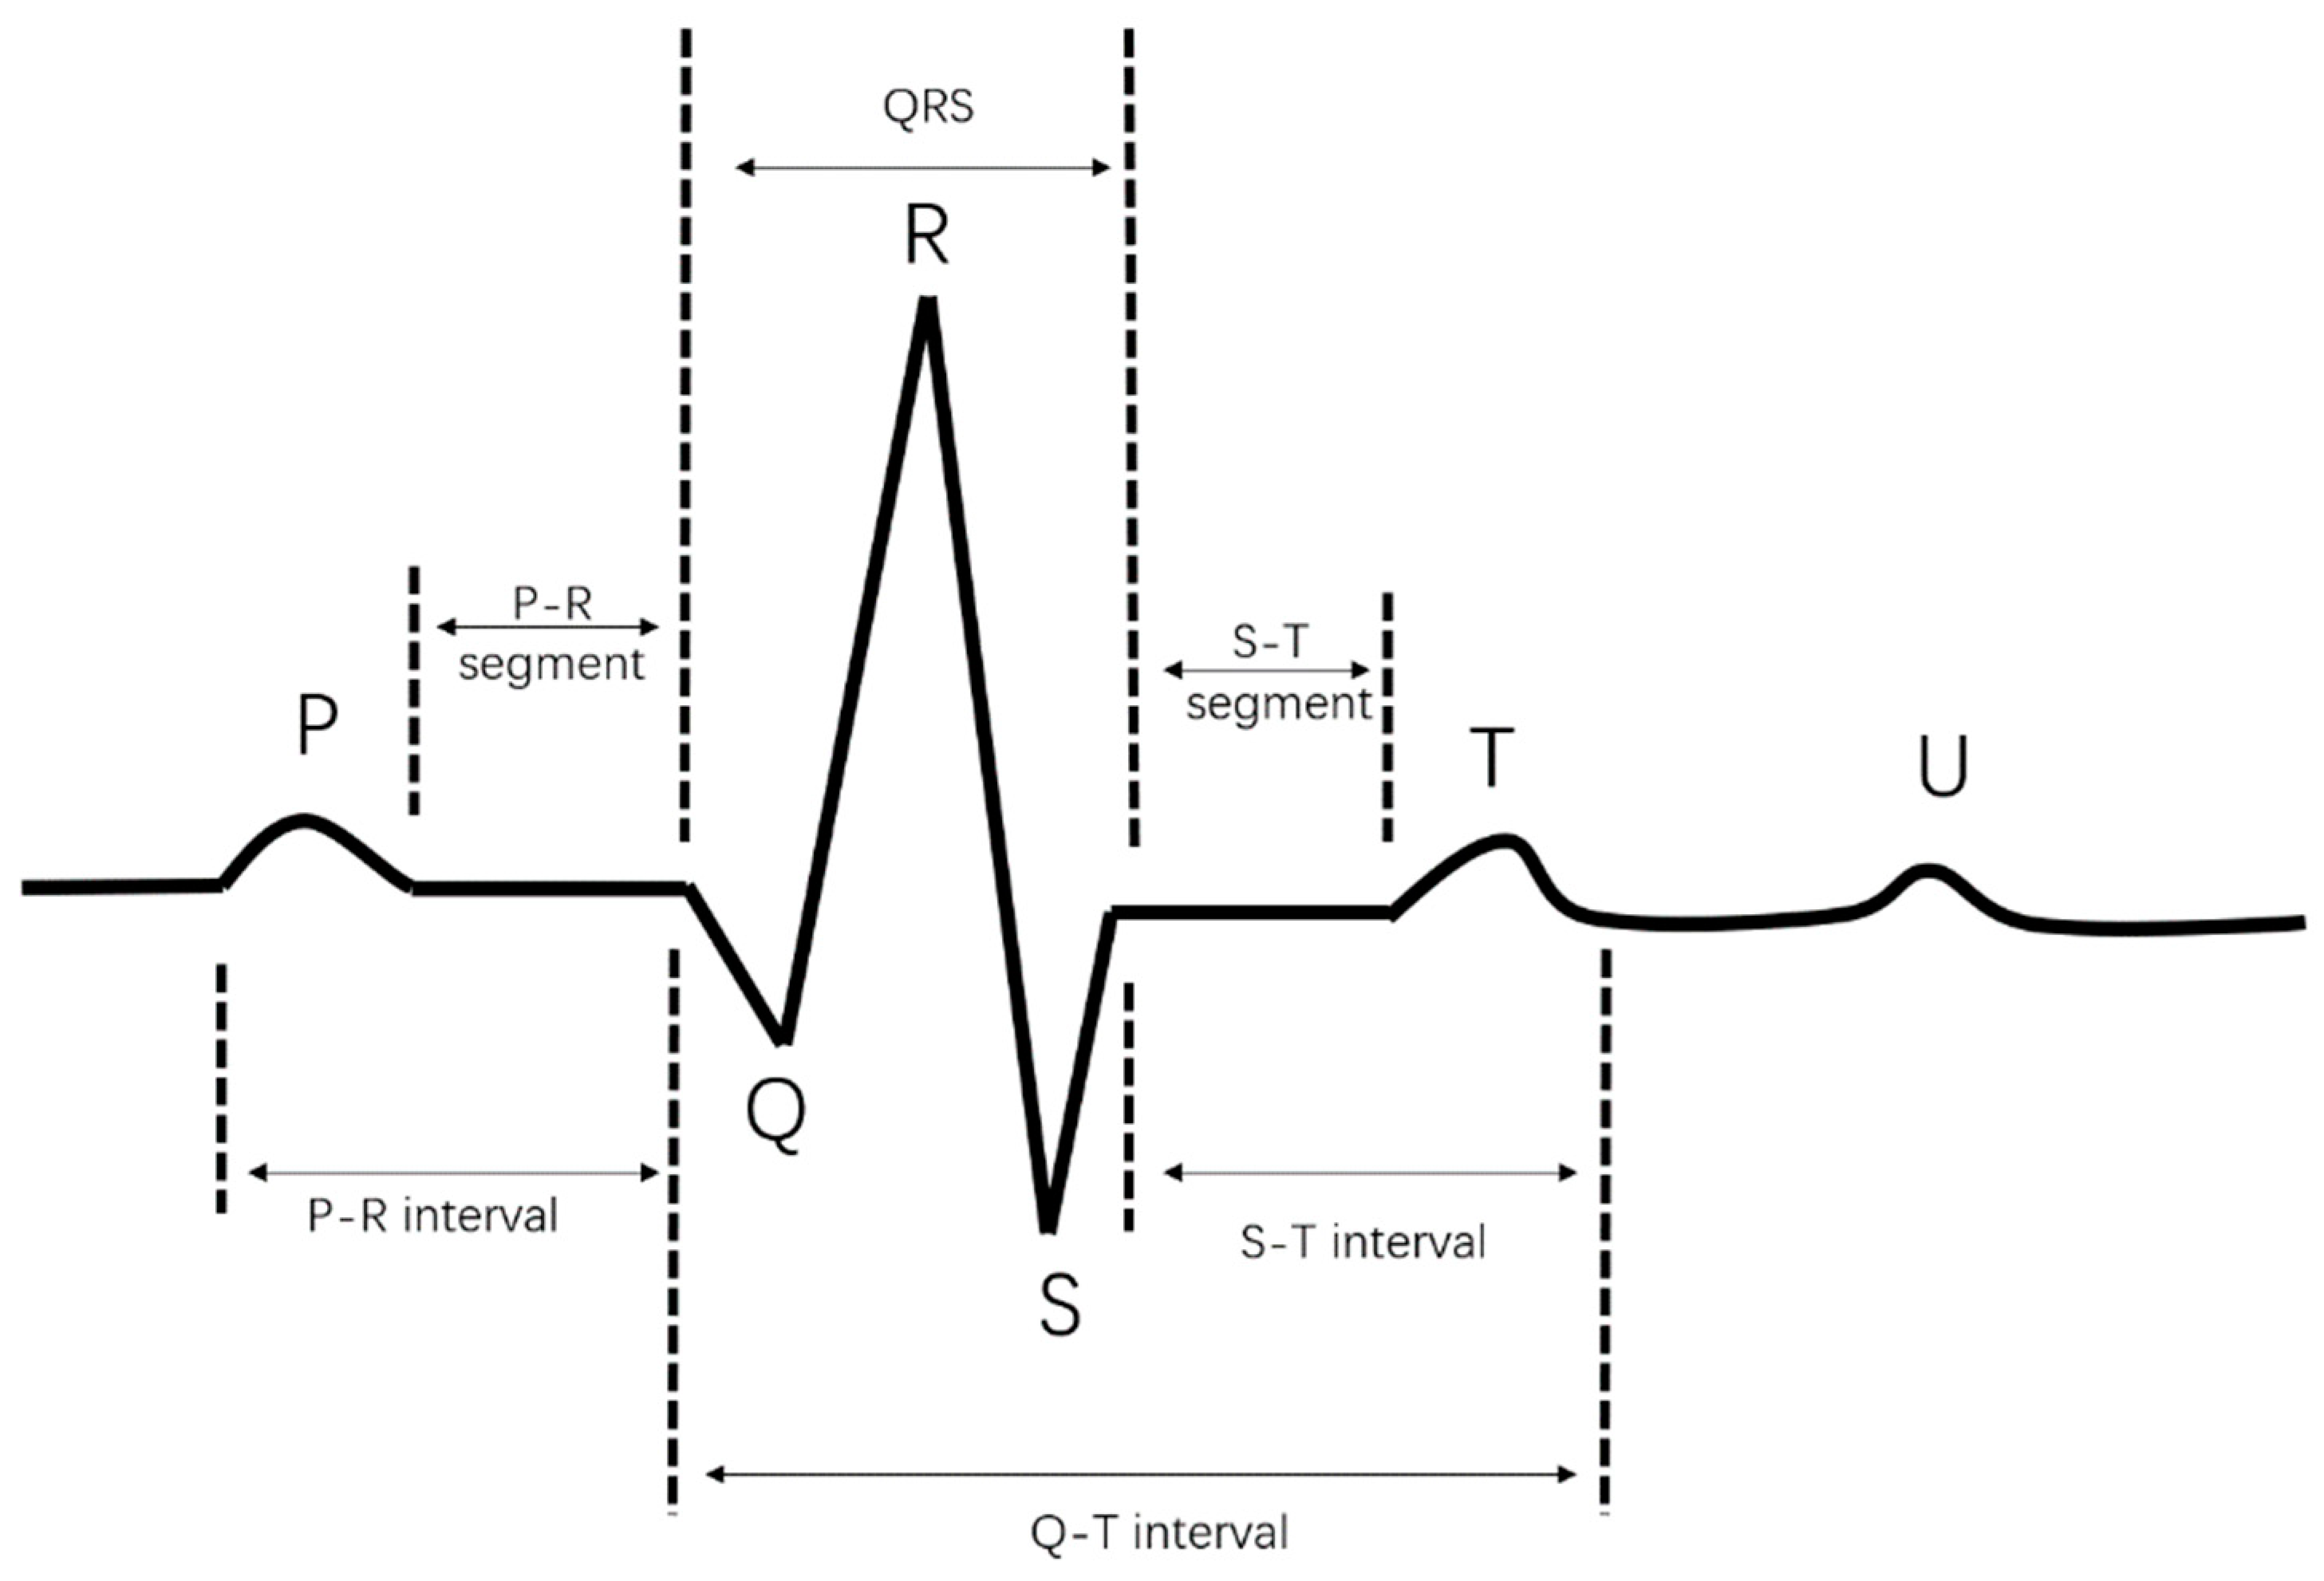
\includegraphics[width=0.8\textwidth]{img/ECG_ondas.png}
        \caption[Ciclo completo de un electrocardiograma]{Ciclo completo de un electrocardiograma\footnotemark}
        \label{fig:ECG_ondas}
    \end{figure}
    \footnotetext{Muestra el ciclo completo de un electrocardiograma, con las ondas P, Q, R, S, T y U, y los intervalos PR, QRS, ST y QT. Imagen tomada de encyclopedia.pub. Fuente: \url{https://encyclopedia.pub/entry/52174}}

    El ECG tiene las características de baja frecuencia y concentración de energía, y la señal es débil, fácilmente perturbada por el ruido, como interferencias eléctricas, campos electromagnéticos externos, movimiento de electrodos (ruido instantáneo)  y el desplazamiento de la línea de base que es causado principalmente por la respiración. Estos ruidos dificultan el diagnóstico médico y pueden provocar errores en la identificación de enfermedades. Por ello, es esencial aplicar técnicas adecuadas para eliminar el ruido y mejorar la calidad de los datos de ECG muestreados. \cite{AlMahamdy_2014}

    \subsection{Fotopletismografía (PPG)}
        \subsubsection{Principios de la fotopletismografía}
            La fotopletismografía (PPG, por sus siglas en inglés) es una técnica óptica que puede utilizarse para detectar cambios en el volumen sanguíneo \cite{Hertzman_1938}. Un PPG es un dispositivo simple que consta de una fuente de luz y un detector; se han desarrollado dispositivos PPG que utilizan luz de diferentes longitudes de onda e intensidades basadas en la tecnología de diodos emisores de luz (LED). La cantidad de energía transferida a la piel por la luz depende de su longitud de onda; por ejemplo, la luz verde se utiliza con frecuencia y tiene una buena relación señal-ruido \cite{Challoner_1979}. Además, las señales de luz roja, verde y azul (RGB) permiten determinar el pulso y las frecuencias respiratorias.

            La función del fotodetector es detectar y cuantificar la luz absorbida durante el flujo pulsátil y no pulsátil. Durante el flujo pulsátil, la luz se absorbe por el cambio en el flujo sanguíneo dentro de las arterias, que es sincrónico con un latido del corazón. Durante el flujo no pulsátil, la luz se absorbe por los tejidos de fondo. Por lo tanto, un fotodetector detecta el cambio volumétrico en el flujo sanguíneo en las arterias al detectar la diferencia de intensidad de luz. La medición de este cambio en la intensidad de la luz ayuda a analizar la funcionalidad del corazón.

            En los últimos treinta años, el número de artículos publicados sobre PPG ha aumentado significativamente, abarcando tanto la investigación básica como la aplicada. En todas estas publicaciones, la PPG ha sido elogiada como una técnica óptica no invasiva, de bajo costo y simple para medir parámetros fisiológicos aplicados en la superficie de la piel. \cite{PPG}.

            La popularidad de este tema se puede atribuir a la comprensión de que la PPG tiene implicaciones importantes para una amplia gama de aplicaciones. Entre muchas, ayuda en la detección de oxígeno en sangre, la evaluación cardiovascular y el control de los signos vitales. Además, la importante contribución de la PPG en los dispositivos portátiles ha elevado exponencialmente la popularidad y la facilidad de uso de la PPG \cite{allen_2007}.

        \subsubsection{Modos de medición}
            La tecnología PPG mide los cambios en el volumen de sangre en los tejidos durante un ciclo cardíaco mediante una fuente de luz. Esta medición volumétrica proporciona información importante sobre el sistema cardiovascular. Un sensor PPG consta principalmente de dos componentes electrónicos: un emisor de luz y un detector de intensidad lumínica.

            Generalmente, se utiliza un LED como emisor de luz y un fotodetector para captar los cambios en la intensidad lumínica. Un pulso PPG correspondiente a un latido del corazón que incluye las fases sistólica y diastólica. Durante la fase sistólica, el corazón se contrae y empuja la sangre rica en oxígeno hacia los tejidos y órganos, lo que incrementa el volumen de sangre en las arterias. Esto provoca que las células sanguíneas absorban más luz, por lo que la cantidad de luz detectada por el fotodetector es menor. En cambio, durante la fase diastólica, el corazón se relaja y la sangre regresa a él, disminuyendo el volumen sanguíneo en las arterias, como resultado, se absorbe menos luz y el fotodetector registra un aumento en la intensidad lumínica.\cite{Hiiberia_2023}.

            Dependiendo de la aplicación y la ubicación del sensor, el PPG se puede usar en modo transmisivo o en modo de reflexión.

            \begin{enumerate}
                \item Cuando un fotodetector y un LED se colocan en lados opuestos de un dedo para detectar la luz transmitida, este arreglo se conoce como modo transmisivo. En este modo, la sonda está configurada de manera que el fotodetector y el LED se enfrentan con una capa de tejido entre ellos. La detección en modo transmisivo depende de la luz que atraviesa las partes del cuerpo, por lo que se prefieren estructuras delgadas como el lóbulo de la oreja y el dedo.
                \item Cuando el fotodetector y el LED se colocan en el mismo lado de un dedo para detectar la luz reflejada, se utiliza el modo reflectivo. En este arreglo, ambos sensores se sitúan uno al lado del otro con una pequeña separación. Por lo tanto, el modo reflectivo puede emplearse en cualquier parte del cuerpo, como la frente o la muñeca.
            \end{enumerate}

            \begin{figure}[H]
                \centering
                \begin{subfigure}[b]{0.45\linewidth}
                    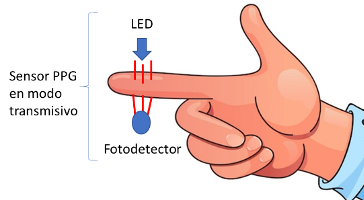
\includegraphics[width=\linewidth]{img/PPG_transmisivo.png}
                    \caption{Sensor PPG en modo de transmisión}
                    \label{fig:PPG_transmisivo}
                \end{subfigure}
                \begin{subfigure}[b]{0.45\linewidth}
                    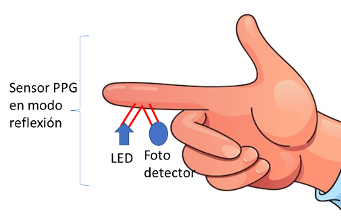
\includegraphics[width=\linewidth]{img/PPG_reflexion.png}
                    \caption{Sensor PPG en modo de reflexión}
                    \label{fig:PPG_reflexion}
                \end{subfigure}
                \caption[Modos de medición de la fotopletismografía]{Modos de medición de la fotopletismografía\footnotemark}
                \label{fig:modosMedicionPPG}
            \end{figure}
            \footnotetext{Muestra la posición de los sensores PPG en modo de transmisión y en modo de reflexión, los dos modo se utiliza para medir la fotopletismografía. Imagen tomada de aiva.hi. Fuente: \url{https://goo.su/pg8UGx}}

            \subsubsection{Forma de onda de un PPG}

            En la figura \ref{fig:PPG} se muestra la señal característica de un fotopletismógrado, la cual está directamente relacionada con la frecuencia cardíaca, donde cada periodo de la señal corresponde a una pulsación del corazon.

            La señal representa dos picos por cada periodo, el pico mayor representa la presión sistólica, y el segundo pico representa el inicio de la presión diastólica cuyo valor es el mínimo de la curva \cite{Celi_2011}.

            Para calcular la frecuencia cardíaca (FC) a partir de la señal PPG, se utiliza la ecuación~\ref{eq:FrecienciaCardiaca}, donde el intervalo entre pico a pico es el tiempo transcurrido entre dos pulsaciones del corazón.

            \begin{equation}
                \label{eq:FrecienciaCardiaca}
                FC = \frac{60}{\textit{Intervalo entre picos}}
            \end{equation}            

            \begin{figure}[H]
                \centering
                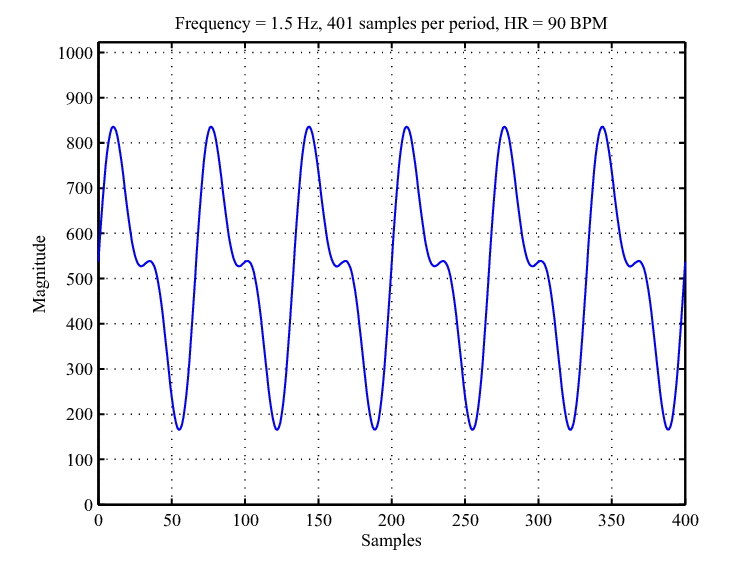
\includegraphics[width=0.7\textwidth]{img/PPG_senial.png}
                \caption[Modelo matemático de una señal pura de una fotopletismografía]{Modelo matemático de una señal pura de una fotopletismografía\footnotemark}
                \label{fig:PPG}
            \end{figure}
            \footnotetext{Muestra una representación de una señal pura de una fotopletismografía, donde se observa la forma de onda de la señal con una frecuencia de 1.5 Hz, que representa 90 latidos por minuto. Imagen tomada del articulo ´´Body sensor network for mobile health monitoring, a diagnosis and anticipating system´´. Fuente: \url{https://doi.org/10.1109/jsen.2015.2464773}}

        
        \subsubsection{Componente AC y DC de la señal PPG}
            La figura \ref{fig:PPG_AC_DC} muestra un ejemplo de una forma de onda fotopletismográfica, que tiene componentes de corriente continua (DC) y corriente alterna (AC). El componente DC de la forma de onda PPG corresponde a la señal óptica transmitida o reflejada del tejido y depende de la estructura del tejido y del volumen promedio de la sangre arterial y venosa. El componente DC cambia lentamente con la respiración, mientras que el componente AC fluctúa de acuerdo con los cambios en el volumen sanguíneo que ocurren entre las fases sistólica y diastólica del ciclo cardíaco \cite{Tamura_2019}.

            Cuando el corazón bombea sangre durante la sístole, el aumento del volumen sanguíneo en los tejidos periféricos provoca una mayor absorción de la luz o una menor reflexión, lo que da lugar a una desviación hacia abajo en la forma de onda PPG. Durante la diástole, cuando el corazón se relaja, el volumen sanguíneo disminuye, lo que da lugar a una desviación hacia arriba en la forma de onda PPG. La tecnología basada en PPG calcula las mediciones en función de los cambios reflejados en la forma de onda \cite{Cabessa_2024}.

            \begin{figure}[H]
                \centering
                \begin{subfigure}[b]{0.45\linewidth}
                    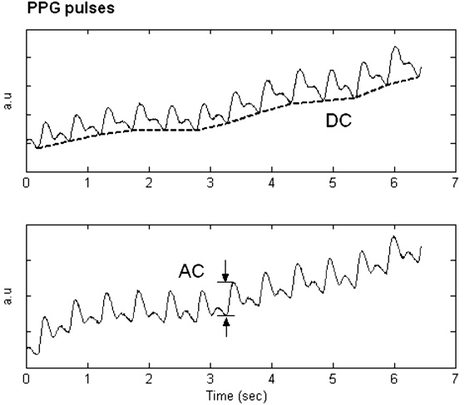
\includegraphics[width=\linewidth]{img/PPG_AC_DC.png}
                \end{subfigure}
                \begin{subfigure}[b]{0.45\linewidth}
                    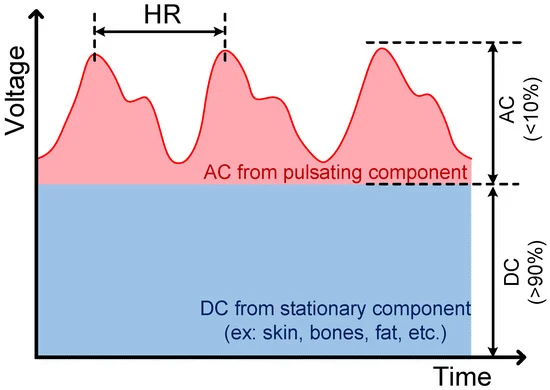
\includegraphics[width=\linewidth]{img/PPG_Componente_AC_DC.png}
                \end{subfigure}
                \caption[Componente AC y DC de la señal PPG]{Componente AC y DC de la señal PPG\footnotemark}
                \label{fig:PPG_AC_DC}
            \end{figure}
            \footnotetext{Muestra un ejemplo de forma de onda de la señal PPG, donde se observa el componente AC y DC de la señal. Imagen tomada del artículo ``Wearable Photoplethysmographic Sensors—Past and Present". Fuente: \url{https://doi.org/10.3390/electronics3020282}}

        \subsubsection{Longitud de onda de la luz emitida}
            La piel del cuerpo está compuesta principalmente por tres capas de tejido: la epidermis, la dermis y la hipodermis. Debido a la absorción, solo las ondas de luz con una longitud de onda mayor pueden penetrar a través de todas ellas. La hemoglobina oxigenada absorbe la luz infrarrojo (NIR), mientras que la hemoglobina desoxigenada absorbe luz en la longitud de onda roja. Como resultado, los PPG que emplean LED y fotodetectores con longitudes de onda NIR y roja se utilizan comúnmente en el control clínico para calcular la concentración de hemoglobina.

            Sin embargo, el movimiento del paciente influye en la precisión de la medición y está relacionado con la longitud de onda de la luz utilizada. La luz de longitud de onda más larga, como el infrarrojo, se ve más afectada por el movimiento debido a que penetra profundamente en el tejido. Por otro lado, la luz de longitud de onda más corta (luz verde) generalmente está libre de los efectos del movimiento, ya que penetra menos en el tejido corporal. Por lo tanto, para mitigar el impacto del movimiento y la absorción de luz por los tejidos, se ha propuesto el uso de PPG basados en sensores ópticos de múltiples longitudes de onda para detectar variaciones en el flujo sanguíneo a diferentes profundidades de la piel. \cite{Hiiberia_2023}.

            \begin{figure}[H]
                \centering
                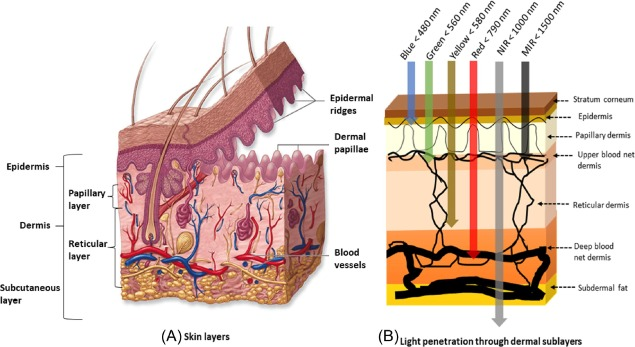
\includegraphics[width=0.8\textwidth]{img/PPG_luz.jpg}
                \caption[Penetración de las longitudes de onda de la luz en la piel]{Penetración de las longitudes de onda de la luz en la piel\footnotemark}
                \label{fig:PPG_longitud_onda}
            \end{figure}
            \footnotetext{Muestra la penetración de la luz en la piel, donde se observa que la luz de longitud de onda más larga (infrarroja) penetra más en la piel que la luz de longitud de onda más corta (Azul). Imagen tomada de Journal of Clinical Monitoring and Computing. Fuente: \url{https://goo.su/jnUP8yi}}

            Dentro de la región visible, el pico de absorción dominante está en la región azul del espectro, seguido de la región verde-amarilla (500-600 nm), correspondiente a los glóbulos rojos. La luz de longitudes de onda más cortas es absorbida fuertemente por la melanina. El agua absorbe la luz en las regiones ultravioleta e infrarroja (IR) más largas. La luz roja (660 nm) e IR (940nm) pasa a través del tejido y la sangre. Por lo tanto, la luz IR se ha utilizado en sensores PPG.
        
            En la última década, la eficiencia de los LED ha aumentado y su voltaje directo ha disminuido, lo que resulta en un mayor número de lúmenes por watt. Gracias a la iluminación de alta potencia, la variación en el ciclo cardíaco entre las fases sistólica y diastólica es más pronunciada en la longitud de onda verde. Por ello, la luz verde se ha empleado en sensores PPG para medir la frecuencia cardíaca y la saturación de oxígeno en la sangre. \cite{Tamura_2019}.

    
    \subsection{Presión Arterial}
    La presión arterial es la fuerza que ejerce la sangre contra las paredes de las arterias. La presión arterial se mide en milímetros de mercurio (mmHg) e incluye dos mediciones: la presión sistólica, que se mide durante el latido del corazón (momento de presión máxima), y la presión diastólica, que se mide durante el descanso entre dos latidos (momento de presión mínima) \cite{PresionArterialDefinicion}.

    La presión arterial normal es de 120/80 mmHg, la presión arterial alta (hipertensión) es de 140/90 mmHg o más y la presión arterial baja (hipotensión) es de 90/60 mmHg o menos \cite{DOF}.